\documentclass[runningheads]{llncs}
%
\usepackage{graphicx}
% Used for displaying a sample figure. If possible, figure files should
% be included in EPS format.
%
% If you use the hyperref package, please uncomment the following line
% to display URLs in blue roman font according to Springer's eBook style:
\usepackage{hyperref}
\renewcommand\UrlFont{\color{blue}\rmfamily}

% User imported packages
\usepackage[utf8]{inputenc}
\usepackage{multirow}
\usepackage{pifont}
\usepackage[backend=biber, style=lncs, maxcitenames=2, maxbibnames=5]{biblatex}
\usepackage{booktabs}
\usepackage{caption, subcaption}
\usepackage{bm}
\usepackage{amsmath}
\usepackage{calc}
\usepackage{amssymb}
\usepackage{cleveref}
\usepackage{todonotes}
\usepackage{varwidth}
\usepackage{tikz}
\usepackage{graphicx}
\newcommand{\cmark}{\ding{51}} % checkmark symbol
\newcommand{\xmark}{\ding{55}} % X-mark symbol

\addbibresource{bibliography.bib}

\begin{document}
%
\title{Supplementary Material: \\Learning Rate Optimization for Online Deep Learning}
%
%\titlerunning{Abbreviated paper title}
% If the paper title is too long for the running head, you can set
% an abbreviated paper title here
%
\author{Anonymous\inst{1}}
%
\authorrunning{Anonymous et al.}
% First names are abbreviated in the running head.
% If there are more than two authors, 'et al.' is used.
%
%\institute{
%    Princeton University, Princeton NJ 08544, USA
%    \and
%    Springer Heidelberg, Tiergartenstr. 17, 69121 Heidelberg, Germany
%    \email{lncs@springer.com}\\
%    \url{http://www.springer.com/gp/computer-science/lncs}
%    \and
%    ABC Institute, Rupert-Karls-University Heidelberg, Heidelberg, Germany\\
%    \email{\{abc,lncs\}@uni-heidelberg.de}
%    }
%

\maketitle

\section*{Hyperparameter Settings for Empirical Evaluation}



\begin{table}[h]
    \centering
    \caption{Parameter Notation as used in Paper.}
    \begin{tabular}{lr}
        \toprule
        Parameter                        & Symbol       \\
        \midrule
        Learning Rate                    & $\eta$       \\
        Decay Factor                     & $\gamma$     \\
        Drift Detection Confidence Level & $\delta$     \\
        Steps Between LR Cycles/Updates  & $s$          \\
        Relative LR at Midpoint of Cycle & $\hat{\eta}$ \\
        \bottomrule
    \end{tabular}
\end{table}
\vspace{-1cm}

\begin{table}[h]
    \centering
    \caption{Search spaces for learning rate.}
    \begin{tabular}{l l}
        \toprule
        Optimizer & Learning Rate Search Space                \\
        \midrule
        SGD       & ${2^1, 2^0, ..., 2^{-8}}$                 \\
        Adam      & ${2^{-3}, 2^{-4}, ..., 2^{-12}}$          \\
        AdaGrad   & ${2^1, 2^0, ..., 2^{-8}}$                 \\
        WNGrad    & ${10^{1.25}, 10^{0.75}, ..., 10^{-7.75}}$ \\
        HD        & ${2^{-3}, 2^{-4}, ..., 2^{-12}}$          \\
        COCOB     & $100$                                     \\
        DoG       & $1$                                       \\
        D-Adapt   & $1$                                       \\
        Mechanic  & $0.01$                                    \\
        \bottomrule
    \end{tabular}
\end{table}
\vspace{-1cm}

\begin{table}[!h]
    \centering
    \caption{Other parameter settings.}
    \begin{tabular}{l l}
        \toprule
        Schedule    & Values                                  \\
        \midrule
        Exponential & $\gamma = 1 - 2^{-13}$                  \\
        Exp. Reset  & $\gamma = 1 - 2^{-12}, \delta = 0.0001$ \\
        Step        & $\gamma = 0.75, s = 2000$               \\
        Cyclic      & $\hat{\eta} = 0.25, s = 8000$           \\
        \bottomrule
    \end{tabular}
\end{table}

\newpage
\section*{Additional Results for Pre-Tuning}


\begin{figure}
    \centering
    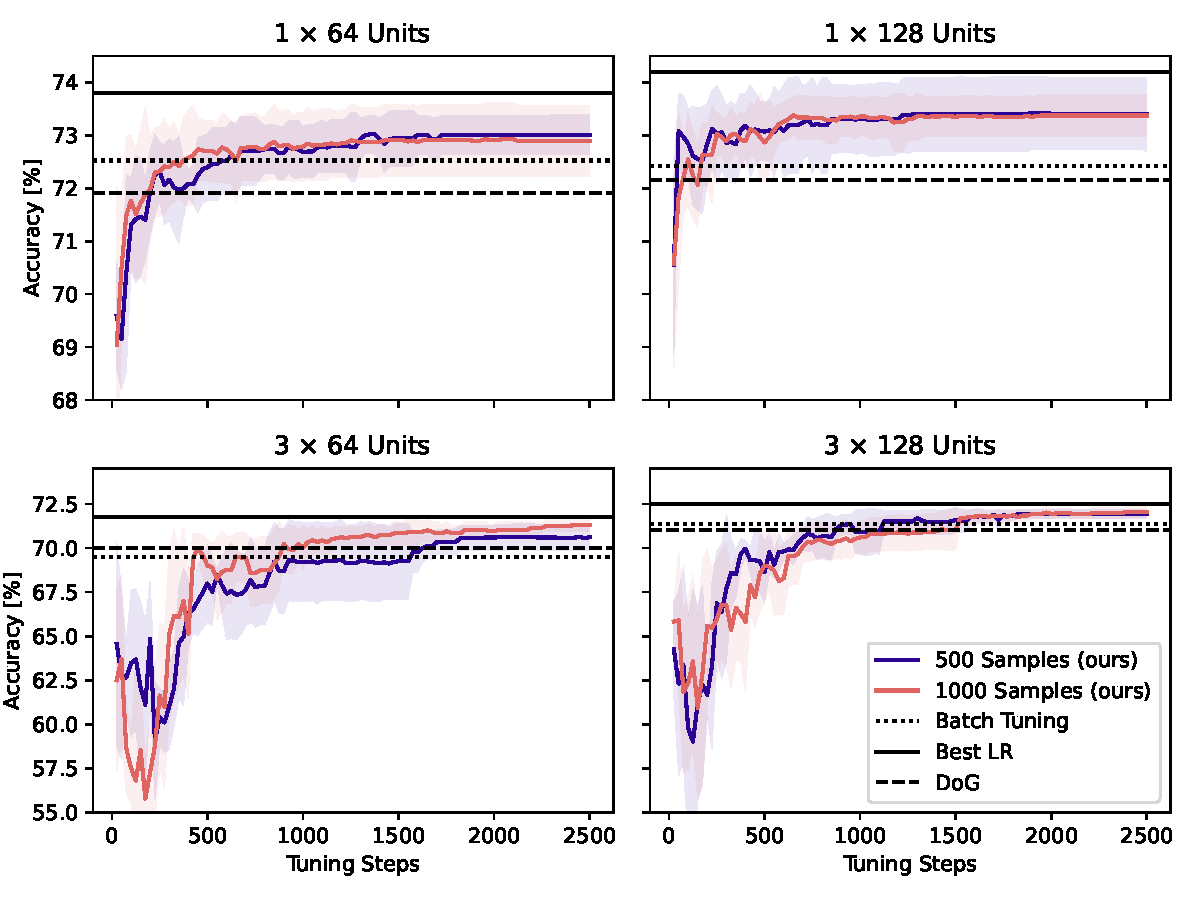
\includegraphics[width=\textwidth]{figures/pretune_architectures_exp_schedule.pdf}
    \caption{Average accuracy over all evalutated real-world datasets achieved by pre-tuning for different network architectures.}
\end{figure}


\end{document}



\end{document}
